\documentclass[12pt]{article}


\title{Power-Index Game Research Write-up}
\date{Aug 2018}
\author{Charlie Gerrie}
\usepackage[utf8]{inputenc}


\usepackage{amsthm}
\usepackage{amsmath}
\usepackage{yfonts}
\usepackage{amssymb}
\usepackage{fullpage}
\usepackage{mathtools}
\usepackage{tikz}
\usepackage{graphicx}
\usepackage{subcaption}
\usepackage{float}
\usepackage{pgf}
\usepackage{url}
\usetikzlibrary{arrows}
\DeclarePairedDelimiter\ceil{\lceil}{\rceil}
\DeclarePairedDelimiter\floor{\lfloor}{\rfloor}
\pagestyle{empty}

\newtheorem{theorem}{Theorem}%[section]

\newtheorem{lemma}{Lemma}%[section]

\newtheorem{proposition}{Proposition}%[section]

\newtheorem{corollary}{Corollary}%[section]

\theoremstyle{definition}
\newtheorem{definition}{Definition}%[section]
 
\theoremstyle{remark}
\newtheorem{remark}{Remark}%[section]

\theoremstyle{remark}
\newtheorem{example}{Example}%[section]

\pagenumbering{gobble}
% TODO SHOULD I HAVE PAGE NUMBERS?

\begin{document}

%TITLE PAGE%
\maketitle
\newpage

%\begin{abstract}
%We examine the power-index game, a cellular automaton, on a torus. 
%\end{abstract}

\tableofcontents

\section{Introduction} \label{IntroSec}

\par
How do people change their mind? How are they affected by others? How does that look in a population? These are all questions that are topical today but people have pondered for centuries. The power-index game is an attempt to model this. It had big goals, but alas, it seems like it will not be used for its intended purpose any time soon. However, its simplicity has given it a new lease at theoretical life as new questions have arisen. % What is the connection between local and global structure? What is the nature of the stability of the game? Why do these simple rules produce the intricate phenomena that we observe? This is the direction in which this research has taken the power-index game.

 

\subsection{The Power Index Game} \label{PIgame}

% explain that it's played on a graph
% define sides (WEAK/STRONG)
% define closed neighborhood
% define together and against sets
% define power
% define iteration behaviour
% explain iteration
\par
What exactly is the power-index game? It is, in short, rules for taking graphs with values on the vertices and iterating them. With zero players, the title of game can seem a misnomer.


% CONTINUE

\begin{definition}[Side]
The set of sides $\mathbb{S}$ is the set containing two elements: strong ($\mathfrak{s}$) and weak ($\mathfrak{w}$). %\textit{These sides will also be associated with and referred to by the colours black and white}.
\end{definition}
\begin{definition}[Configuration]
A configuration is a mapping $C\colon V \to \mathbb{S}$, where $V$ is the vertex set of a graph. \cite{ref:graphs}. 
\end{definition}
\begin{definition}[Game]
A game $G(B,C)$ is a structure composed of both a graph $B(V,E)$ (as in board) with associated vertex and edge sets $V$ and $E$, and a configuration $C$, which assigns a side to each vertex.
\end{definition}
\begin{remark}
We will often refer to vertices as black or white instead of strong or weak, respectively, because those are the colours we use to display them on tori. This is discussed further in section \ref{Simplification}.
\end{remark}

\begin{definition}[Iteration operator]
We define an operator $I$ which acts on a game to iterate it. % For example, $IG$ would be the game $G$ iterated once, and $I^n G$ would be it iterated $n$ times.
\end{definition}

% SHOULD I GIVE AN EXAMPLE?



\subsection{Prior Work and Variations} \label{PriorWork}
% SHAPLEY AND SHUBIK
\par
The idea of the power-index was started by Lloyd Shapley and Martin Shubik. \cite{ref:PowerIndex} They developed it to model voting behavior. This was the inspiration for the Power-Index Game in its current iteration, which was developed by Richard Nowakowski.
% WHAT THEY FOUND
\par
The idea of the power-index is that every cell is assigned a power based on its neighborhood, and that determines how it is able to affect its neighbors. In its current form, it is defined like this:
\begin{equation}
	P(v) =
	\begin{cases}
		\begin{cases}
			\frac{1}{|A|} & \text{if\ } |A|>|D| \\
			0 & \text{if\ } |D|\geq|A|
		\end{cases} & \text{If\ }C(v)=\mathfrak{w} \\
		\begin{cases}
			\frac{1}{|A|} & \text{if\ } |A|\geq |D| \\
			0 & \text{if\ } |D|> |A|
		\end{cases} & \text{If\ }C(v)=\mathfrak{s}
	\end{cases}
\end{equation}
Where $v$ is a vertex, $P(v)$ is its power, $C$ is a configuration, and $\mathfrak{s}$ and $\mathfrak{w}$ are strong and weak sides.
\par
Previous work on the power-index game in its current incarnation was done by Jordan Barrett and Richard Nowakowski. One of their main results of note was discovering a construction for arbitrarily large cycles. We reconfirm this result in section \ref{Astakos}. They also examined the game on many different boards. We, however, will limit ourselves to only one type of board: tori.

% CONTINUE

% WHAT I AM INTERESTED IN / CONNECTIONS TO THIS WORK

%\subsection{Improvements on Prior Results} \label{Improvements}
% ARBITRARY CYCLES (SHOULD THIS BE IN THE "POWER INDEX ON A TORUS" SECTION?)
% motivate arbitrary cycles
%\par
%Recall that one of the previous results was arbitrarily large cycles. This raises the question of if cycles of any specific length can occur in the game. We have found a construction that demonstrates that this is possible.
% show initial conditions for astakos
%\par
%Consider the following configuration on a torus % smallest astakos
%This construction can be generalized to a $3\times n$ torus which corresponds to a cycle length of $n$. 
% show that it iterates and loops (make sure you mention that it's on a torus)
% result: arbitrary cycles are possible

\section{The Power Index Game on a Torus} \label{Main Chapter}
%mention toroidal grid
\subsection{Simplifications} \label{Simplification}
\begin{definition}[Torus]
An $n$-by-$m$ torus is the cartesian graph product of an $n$-cycle and an $m$-cycle. Informally, it is a grid where the edges wrap around.
\end{definition}

% motivation
\par
The rules of the game can be restated in simpler terms when limited to a torus. All of the tori we have used have been toroidal grids, so the graphs are 4-regular. Thus, the rules from \ref{PIgame} for the power can be simplified to a simple 1-neighborhood cellular automaton with the following rules:
% definitions
% power
\begin{equation}
	\label{powerEq}
	P(v) =
	\begin{cases}
		\frac{1}{3} & \text{if $|A(v)|=2$} \\
		\frac{1}{4} & \text{if $|A(v)|=3$} \\
		\frac{1}{5} & \text{if $|A(v)|=4$} \\
		0 & \text{if $|A(v)|\in \{0,1\}$}
	\end{cases}
\end{equation}
\begin{figure}[H]
	\centering
	\begin{subfigure}[b]{0.1\linewidth}
	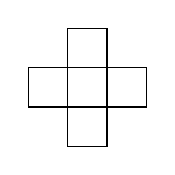
\begin{tikzpicture}
		\draw(0,0.5) rectangle (0.5,1);
		\draw(0.5,0) rectangle (1,0.5);
		\draw(0.5,0.5) rectangle (1,1);					% REPEAT ME!
		\draw(0.5,1) rectangle (1,1.5);
		\draw(1,0.5) rectangle (1.5,1);
	\end{tikzpicture}
	\caption{$\frac{1}{5}\ power$}
	\end{subfigure}
	\begin{subfigure}[b]{0.1\linewidth}
	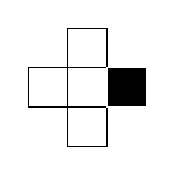
\begin{tikzpicture}
		\draw(0,0.5) rectangle (0.5,1);
		\draw(0.5,0) rectangle (1,0.5);
		\draw(0.5,0.5) rectangle (1,1);					% REPEAT ME! AND SPACE THEM!
		\draw(0.5,1) rectangle (1,1.5);
		\path[draw=white,fill=black] (1,0.5) rectangle (1.5,1);
	\end{tikzpicture}
	\caption{$\frac{1}{4}\ power$}
	\end{subfigure}
	\begin{subfigure}[b]{0.1\linewidth}
	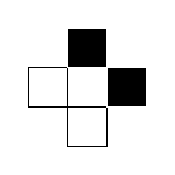
\begin{tikzpicture}
		\draw(0,0.5) rectangle (0.5,1);
		\draw(0.5,0) rectangle (1,0.5);
		\draw(0.5,0.5) rectangle (1,1);					% REPEAT ME!
		\path[draw=white,fill=black] (0.5,1) rectangle (1,1.5);
		\path[draw=white,fill=black] (1,0.5) rectangle (1.5,1);
	\end{tikzpicture}
	\caption{$\frac{1}{3}\ power$}
	\end{subfigure}
	\begin{subfigure}[b]{0.1\linewidth}
	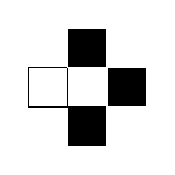
\begin{tikzpicture}
		\draw(0,0.5) rectangle (0.5,1);
		\path[draw=white,fill=black] (0.5,0) rectangle (1,0.5);
		\draw(0.5,0.5) rectangle (1,1);					% REPEAT ME!
		\path[draw=white,fill=black] (0.5,1) rectangle (1,1.5);
		\path[draw=white,fill=black] (1,0.5) rectangle (1.5,1);
	\end{tikzpicture}
	\caption{$0\ power$}
	\end{subfigure}
	\begin{subfigure}[b]{0.1\linewidth}
	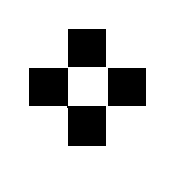
\begin{tikzpicture}
		\path[draw=white,fill=black] (0,0.5) rectangle (0.5,1);
		\path[draw=white,fill=black] (0.5,0) rectangle (1,0.5);
		\draw(0.5,0.5) rectangle (1,1);					% REPEAT ME!
		\path[draw=white,fill=black] (0.5,1) rectangle (1,1.5);
		\path[draw=white,fill=black] (1,0.5) rectangle (1.5,1);
	\end{tikzpicture}
	\caption{$0\ power$}
	\end{subfigure}
	\caption{all possible neighborhoods for a center cell}
	\label{neighHeurs}
\end{figure}

% next iteration?
	
% results
	% explain 2-neighborhood
	
% % % % SYMMETRIES!
\subsection{Symmetries}

\par
Before we dive fully into the power-index game, we should take a moment to examine the symmetries present. First of all, the rules of the game are rotationally invariant. The power of a given cell only depends on the number of neighbors of particular sides,
not where they are, and the % some problem here?
process for finding the most powerful neighbor is similar. Thus, this symmetry will be used often to reduce cases. However, one must be careful about applying this symmetry where it does not apply. There are many occasions where we will deal with larger-scale structures where rotational symmetry does not apply, or worse it is invoked as an approximation (see \ref{2squareFirst}). Translational and reflective symmetries are also present for similar reasons to rotational symmetry, and so share the same potential pitfalls.

\par
The final symmetry of the power-index game is that of the sides. Recall that sides are the values of strong or weak that are assigned to vertices on the graph the game is being played on. This applies because we are limiting ourselves to tori, which are 4-regular. Normally, strong would break ties for the majority of the closed neighborhood, but the closed neighborhoods of cells on tori have five cells, so ties are not a problem. Thus, strong and weak are equivalent and can be exchanged freely.
% SIDE
% ROTATIONAL
% TRANSLATIONAL
% MIRROR

\subsection{Examples}
\par
Let us examine an example of how to iterate the game. In figure \ref{exampleIter}, we see a single cell in the center, and all cells within 2 moves from it, which is the maximum distance away that a cell can affect another during one iteration. We denote this area the \emph{2-neighborhood}, because it is the neighborhood of cells 2 away from a cell. In the figure, we see the powers of each of cell immediately around the center. We calculate these with equation \ref{powerEq}. The center cell will change to the side of the most powerful neighbor. There are two cells tied for most powerful on its left and its right. In this case, the cell will go with its own side and stay the same if possible. Thus, this cell will not change in the next iteration.
\begin{figure}
	\centering
	\label{exampleIter}
	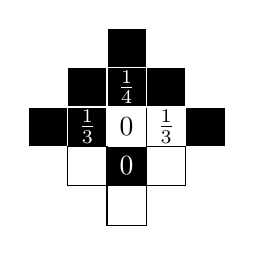
\begin{tikzpicture}
		\path[draw=black,fill=white] (0,0) rectangle (0.5,0.5);
		\path[draw=white,fill=black] (-0.5,0) rectangle (0,0.5);
		\path[draw=white,fill=black] (-1,0) rectangle (-0.5,0.5);
		\path[draw=black,fill=white] (0.5,0) rectangle (1,0.5);
		\path[draw=white,fill=black] (1,0) rectangle (1.5,0.5);
		\path[draw=white,fill=black] (0,0.5) rectangle (0.5,1);
		\path[draw=white,fill=black] (0.5,0.5) rectangle (1,1);
		\path[draw=white,fill=black] (-0.5,0.5) rectangle (0,1);
		\path[draw=white,fill=black] (0,1) rectangle (0.5,1.5);
		\path[draw=white,fill=black] (0,-0.5) rectangle (0.5,0);
		\path[draw=black,fill=white] (-0.5,-0.5) rectangle (0,0);
		\path[draw=black,fill=white] (0.5,-0.5) rectangle (1,0);
		\path[draw=black,fill=white] (0,-1) rectangle (0.5,-0.5);
		
		\node[text=black,align=center] at (0.25,0.25) {0};
		\node[text=white,align=center] at (-0.25,0.25) {$\frac{1}{3}$};
		\node[text=white,align=center] at (0.25,0.75) {$\frac{1}{4}$};
		\node[text=white,align=center] at (0.25,-0.25) {0};
		\node[text=black,align=center] at (0.75,0.25) {$\frac{1}{3}$};
	\end{tikzpicture}
	\caption{}
\end{figure}
% help people get a sense of how the game goes

\subsection{Special Shapes} \label{SpecialShapes}

\par
Recall the definition of a configuration from section \ref{PIgame}. In short, a configuration is a particular assignment of sides to every vertex of the game board. 
% motivation

%\begin{definition}[Configuration]
%A configuration is a particular side state of an entire graph.
%A configuration is a mapping from a board ()
%\end{definition}
% EXAMPLES

\begin{definition}[Subconfiguration]
%A subconfiguration is an arrangement of cells, irrespective of its surrounding configuration.
A subconfiguration is a configuration of a subgraph of the board of a game.
\end{definition}
% EXAMPLES
\begin{example}
Three adjacent cells in a row, where the center one is strong and the other two are weak can be a subconfiguration, in the sense that another graph can contain such an arrangement on a particular part of the board.
\end{example}

% results of these definitions

\subsubsection{On An Empty Grid} \label{EmptyGrid}
\par
These shapes are considered to be simulated on a grid of entirely the opposite colour, devoid of any other patterns.

\begin{definition}[Unstable Subconfiguration]
A configuration is called unstable if there exists a finite number of iterations after which it will die out, and the grid returns to homogeneity. 
\end{definition}
\begin{example}
A chevron is an unstable subconfiguration, since it dies out after two iterations.

%FIGURES

\end{example}


\begin{definition}[Stable Subconfiguration]
A configuration is called stable if there exists a finite number of iterations after which it will be reproduced. 
\end{definition}
\begin{example}
A 3-by-3 square is a stable subconfiguration, since if it is placed in a field of the opposite colour it will form a cycle of length 3. See figure \ref{StableConfigs}.

\begin{figure}
  \centering
  \begin{subfigure}[b]{0.4\linewidth}
    %\includegraphics[width=\linewidth]{3x3_1.png}
    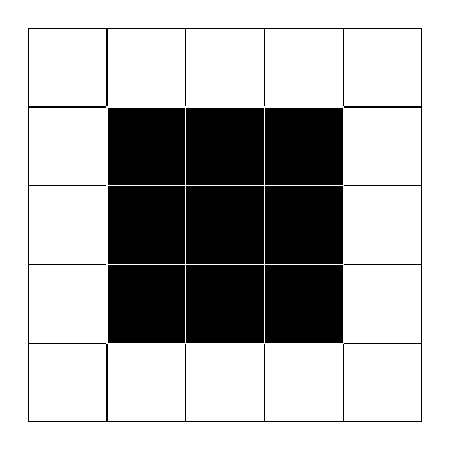
\begin{tikzpicture}
      \foreach \x in {1,...,5} {
        \foreach \y in {1,...,5} {
          \draw(\x,\y) rectangle (1+\x,1+\y);
        }
      }
      \foreach \x in {2,...,4} {
        \foreach \y in {2,...,4} {
          \path[draw=white,fill=black] (\x,\y) rectangle (1+\x,1+\y);
        }
      }
    \end{tikzpicture}
    \caption{Iteration 1}
    \label{fig:3x3_1}
  \end{subfigure}
  \begin{subfigure}[b]{0.4\linewidth}
    %\includegraphics[width=\linewidth]{3x3_2.png}
    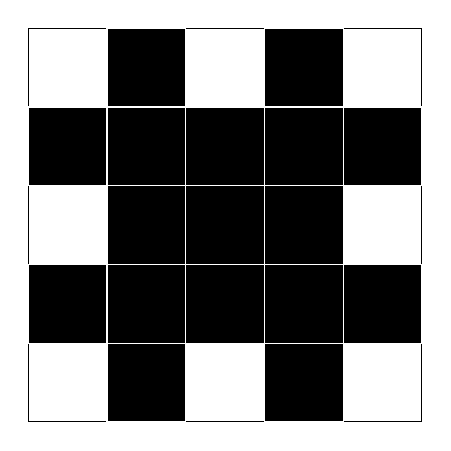
\begin{tikzpicture}
      \foreach \x in {0,...,4} {
        \foreach \y in {0,...,4} {
          \draw(\x,\y) rectangle (1+\x,1+\y);
        }
      }
      \foreach \x in {1,...,3} {
        \foreach \y in {1,...,3} {
          \path[draw=white,fill=black] (\x,\y) rectangle (1+\x,1+\y);
        }
      }
      \path[draw=white,fill=black] (0,1) rectangle (1,2);
      \path[draw=white,fill=black] (0,3) rectangle (1,4);
      \path[draw=white,fill=black] (1,0) rectangle (2,1);
      \path[draw=white,fill=black] (3,0) rectangle (4,1);
      \path[draw=white,fill=black] (1,4) rectangle (2,5);
      \path[draw=white,fill=black] (3,4) rectangle (4,5);
      \path[draw=white,fill=black] (4,1) rectangle (5,2);
      \path[draw=white,fill=black] (4,3) rectangle (5,4);
    \end{tikzpicture}
    \caption{Iteration 2}
    \label{fig:3x3_2}
  \end{subfigure}
  \begin{subfigure}[b]{0.4\linewidth}
    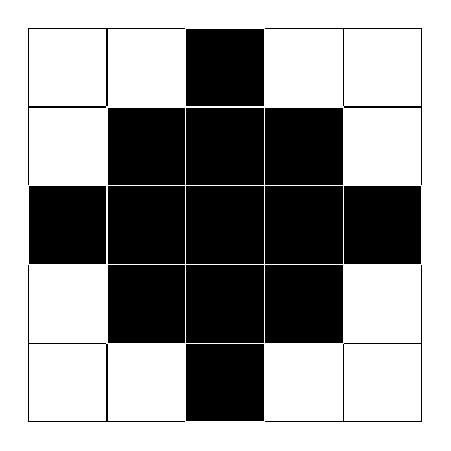
\begin{tikzpicture}
      \foreach \x in {0,...,4} {
        \foreach \y in {0,...,4} {
          \draw(\x,\y) rectangle (1+\x,1+\y);
        }
      }
      \foreach \x in {1,...,3} {
        \foreach \y in {1,...,3} {
          \path[draw=white,fill=black] (\x,\y) rectangle (1+\x,1+\y);
        }
      }
      \path[draw=white,fill=black] (0,2) rectangle (1,3);
      \path[draw=white,fill=black] (4,2) rectangle (5,3);
      \path[draw=white,fill=black] (2,0) rectangle (3,1);
      \path[draw=white,fill=black] (2,4) rectangle (3,5);
    \end{tikzpicture}
    \caption{Iteration 3}
    \label{fig:3x3_3}
  \end{subfigure}
  \begin{subfigure}[b]{0.4\linewidth}
    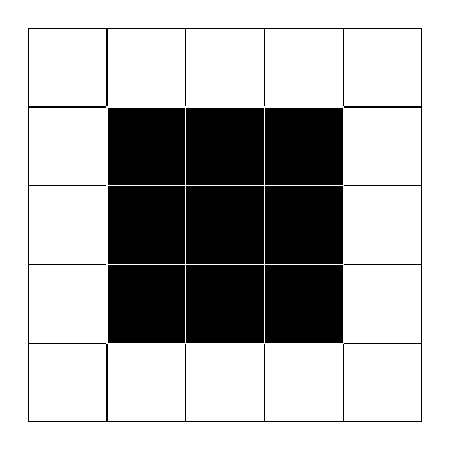
\begin{tikzpicture}
      \foreach \x in {1,...,5} {
        \foreach \y in {1,...,5} {
          \draw(\x,\y) rectangle (1+\x,1+\y);
        }
      }
      \foreach \x in {2,...,4} {
        \foreach \y in {2,...,4} {
          \path[draw=white,fill=black] (\x,\y) rectangle (1+\x,1+\y);
        }
      }
    \end{tikzpicture}
    \caption{Iteration 4}
    \label{fig:3x3_4}
  \end{subfigure}
  \caption{3-by-3 square on a 12-by-12 torus}
  \label{StableConfigs}
\end{figure}



%FIGURES

\end{example}
\begin{remark}
The 5-by-5 and 7-by-7 square are also stable. This sparked the idea that maybe all odd squares above 2 were stable. This hypothesis was quickly disproven by considering the 9-by-9 square, which is parastable.
\end{remark}

\begin{definition}[Parastable Subconfiguration]
A configuration is called parastable if it doesn't die out, but instead fills its space with stable patterns.
\end{definition}
\begin{example}
A 2-by-2 square is a parastable subconfiguration. See figure \ref{ParastableFig}.

\begin{figure}
  \centering
  \begin{subfigure}[b]{0.25\linewidth}
    \includegraphics[width=\linewidth]{2x2_1.png}
    \caption{Iteration 1}
    \label{fig:2x2_1}
  \end{subfigure}
  \begin{subfigure}[b]{0.25\linewidth}
    \includegraphics[width=\linewidth]{2x2_2.png}
    \caption{Iteration 2}
    \label{fig23x2_2}
  \end{subfigure}
  \begin{subfigure}[b]{0.25\linewidth}
    \includegraphics[width=\linewidth]{2x2_3.png}
    \caption{Iteration 3}
    \label{fig:2x2_3}
  \end{subfigure}
  \begin{subfigure}[b]{0.25\linewidth}
    \includegraphics[width=\linewidth]{2x2_20.png}
    \caption{Iteration 20}
    \label{fig:2x2_20}
  \end{subfigure}
  \begin{subfigure}[b]{0.25\linewidth}
    \includegraphics[width=\linewidth]{2x2_50.png}
    \caption{Iteration 50}
    \label{fig:2x2_50}
  \end{subfigure}
  \begin{subfigure}[b]{0.25\linewidth}
    \includegraphics[width=\linewidth]{2x2_100.png}
    \caption{Iteration 100}
    \label{fig:2x2_100}
  \end{subfigure}
  \caption{2-by-2 square on a 60-by-60 torus}
  \label{ParastableFig}
\end{figure} 

\end{example}
\begin{example}
Consider the tetrominoes. All subconfigurations with less than four cells are unstable, so these are the first ones to exhibit parastability. Though the S, Z, and T tetrominoes are unstable, the L, I, and O tetrominoes are all parastable. % DIAGRAMS OF THEM
\begin{figure}
  \centering
  \begin{subfigure}[b]{0.4\linewidth}
    \fbox{\includegraphics[width=\linewidth]{Lstart.png}}
    \caption{iteration 1}
  \end{subfigure}
  \begin{subfigure}[b]{0.4\linewidth}
    \fbox{\includegraphics[width=\linewidth]{Lend.png}}
    \caption{iteration 93}
  \end{subfigure}
  \caption{L tetromino}
\end{figure}
\end{example}

\par
Not much is understood about the mechanism of parastability at this time. However, for large subconfigurations, it appears that stability or instability are the exceptions whereas parastability is the rule.

\subsubsection{A Glider} \label{Astakos}
\par
We have discovered a construction to have a cycle of arbitrary length greater or equal to 6. See figure \ref{Astakos}.

% DIAGRAM SHOWING POWERS

\begin{figure}
  \centering
  \begin{subfigure}[b]{0.25\linewidth}
    \fbox{\includegraphics[width=\linewidth]{astakos1.png}}
    \caption{Iteration 1}
  \end{subfigure}
  \begin{subfigure}[b]{0.25\linewidth}
    \fbox{\includegraphics[width=\linewidth]{astakos2.png}}
    \caption{Iteration 2}
  \end{subfigure}
  \begin{subfigure}[b]{0.25\linewidth}
    \fbox{\includegraphics[width=\linewidth]{astakos3.png}}
    \caption{Iteration 3}
  \end{subfigure}
  \begin{subfigure}[b]{0.25\linewidth}
    \fbox{\includegraphics[width=\linewidth]{astakos4.png}}
    \caption{Iteration 4}
  \end{subfigure}
  \begin{subfigure}[b]{0.25\linewidth}
    \fbox{\includegraphics[width=\linewidth]{astakos5.png}}
    \caption{Iteration 5}
  \end{subfigure}
  \begin{subfigure}[b]{0.25\linewidth}
    \fbox{\includegraphics[width=\linewidth]{astakos6.png}}
    \caption{Iteration 6}
  \end{subfigure}
  \begin{subfigure}[b]{0.25\linewidth}
    \fbox{\includegraphics[width=\linewidth]{astakos1.png}}
    \caption{Iteration 7}
  \end{subfigure}
  \caption{The glider}
  \label{Astakos}
\end{figure}

\begin{theorem}
The power-index game is capable of having arbitrary cycles.
\end{theorem}
\begin{proof}
Cycles of length 1 through 5 are trivial. All larger cycles of length $n$ can be constructed by placing a glider on a $3$-by-$n$ board.
\end{proof}
\begin{remark}
We dubbed the glider "\textit{astakos}", after the Greek work for lobster.
\end{remark}

\subsubsection{Uniform Power Configurations} \label{UPCs} %ACTUALLY USE THIS ACCRONYM?
\begin{definition}[Uniform Power Configuration (UPC)]
A configuration where every cell has the same power.
\end{definition}
\par
We consider UPCs because they will always be static; For a cell to change it would have to have a more powerful neighbor. On a torus, there are four options for the power of a cell: $0$, $\frac{1}{3}$, $\frac{1}{4}$, and $\frac{1}{5}$. % CHECK "HAVE" SYNTAX -_-

\par
The first of these which we will consider is configurations with a uniform power of $\frac{1}{5}$, since they are the simplest. For a cell to have a power of $\frac{1}{5}$, it must be surrounded entirely by neighbors of its own side. Thus, such configurations must be made up of entirely one colour. This type of configuration can be made on a torus of any dimensions.

\par
% rewrite this as opposing or opposite side?
Next, we will consider those with a power of $\frac{1}{4}$. In this case, every cell must have one neighbor of the opposite side. Thus, we can inductively construct what this configuration will look like by starting with a single cell.
% FIGURE OF A CELL WITH A 1-NEIGHBORHOOD WITH ALL BUT THE RIGHT CELL BEING THE WHITE
% LABEL THE RIGHT ONE R, AND THE ONES ABOVE AND BELOW R AS a AND b
\begin{figure}[H]
	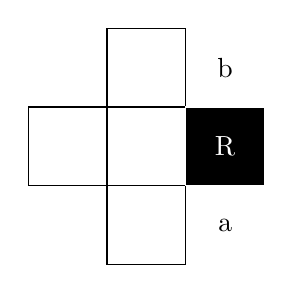
\begin{tikzpicture}
		\draw(0,1) rectangle (1,2);
		\draw(1,0) rectangle (2,1);
		\draw(1,1) rectangle (2,2);					% REPEAT ME!
		\draw(1,2) rectangle (2,3);
		\path[draw=white,fill=black] (2,1) rectangle (3,2);
		
		\node[text=white,align=center] at (2.5,1.5) {R};
		\node[align=center] at (2.5,0.5) {a};
		\node[align=center] at (2.5,2.5) {b};
	\end{tikzpicture}
\end{figure}
Now, we know that the spaces to at $a$ and $b$ must be the same side as $R$, because if they were not, then $R$ would have two neighbors of the opposite side.
\begin{figure}[H]
	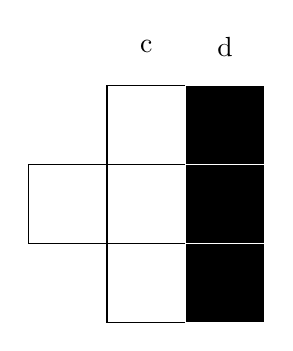
\begin{tikzpicture}
		\draw(0,1) rectangle (1,2);
		\draw(1,0) rectangle (2,1);
		\draw(1,1) rectangle (2,2);
		\draw(1,2) rectangle (2,3);
		\path[draw=white,fill=black] (2,1) rectangle (3,2);
		\path[draw=white,fill=black] (2,0) rectangle (3,1);
		\path[draw=white,fill=black] (2,2) rectangle (3,3);
		
		\node[align=center] at (1.5,3.5) {c};
		\node[align=center] at (2.5,3.5) {d};
	\end{tikzpicture}
\end{figure}
Now we see that $c$ and $d$ must be coloured the same colour as the cells below them. We can continue this type of argument upwards and downwards, forming stripes.
% FIGURE OF TWO ADJACENT 2-STRIPES WITH DOMAINS LEFT AND RIGHT LABELLED L AND R
\begin{figure}[H]
	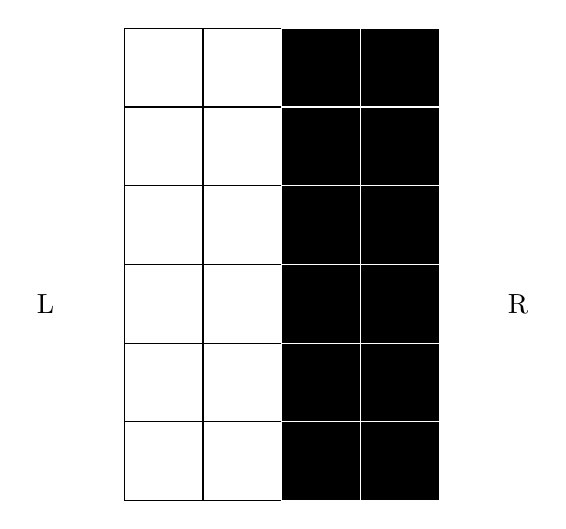
\begin{tikzpicture}
		\foreach \i in {0,...,5} {
		\draw(0,\i) rectangle (1,1+\i);
		\draw(1,\i) rectangle (2,1+\i);
		\path[draw=white,fill=black] (2,\i) rectangle (3,1+\i);
		\path[draw=white,fill=black] (3,\i) rectangle (4,1+\i);
		}
		
		
		\node[align=center] at (-1,2.5) {L};
		\node[align=center] at (5,2.5) {R};
	\end{tikzpicture}
\end{figure}

Finally, we see that the domains $L$ and $R$ must be black and white. Thus, we can continue this pattern to the left and right.
% FINAL FIGURE
We call this pattern a tessellation of 2-stripes, since each stripe is two cells wide. This configuration has a limitation on its dimensions. In this case, the width must be a multiple of 4 to accommodate the repeating pattern of the 2-stripes. So, for example, a UPC could not exist on a 3-by-5 torus, but one could exist on a 3-by-4 torus. On tori where both dimensions are multiples of 4, the stripes can be placed in either orientation.

\par
% UPC OF 0 POWER
UPCs of power $0$ are somewhat more complicated than the previous ones. First off, the trivial solution to having a board with uniform power $0$ is a checkerboard pattern, where every cell has zero neighbors on its side. Note that checkerboard configurations can only exist on even-by-even tori. See figure \ref{Checkerboard} for an example. 
\begin{figure}
  \centering
  \fbox{\includegraphics[width=0.5\linewidth]{checkers.png}}
  \caption{Checkerboard configuration}
  \label{Checkerboard}
\end{figure}
\par
However, cells will also have power $0$ if they have one neighbor on the same side. In this case, we can use the inductive method we used for $\frac{1}{4}$-power. Start with a single cell.
% DIAGRAM OF SINGLE CELL WITH UPPER, LEFT, AND BELOW CELLS THE OPPOSITE COLOUR. LABEL CENTRE S AND RIGHT CELL a
\begin{figure}[H]
	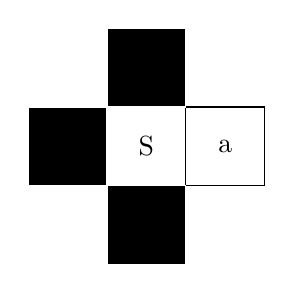
\begin{tikzpicture}
		\path[draw=black,fill=white] (0,0) rectangle (1,1);
		\path[draw=black,fill=white] (1,0) rectangle (2,1);
		\path[draw=white,fill=black] (-1,0) rectangle (0,1);
		\path[draw=white,fill=black] (0,1) rectangle (1,2);
		\path[draw=white,fill=black] (0,-1) rectangle (1,0);
		
		\node[align=center] at (0.5,0.5) {S};
		\node[align=center] at (1.5,0.5) {a};
	\end{tikzpicture}
\end{figure}
Next we can fill in the neighbors of $a$.
% DIAGRAM WITH RIGHT CELL NEIGHBORHOOD FILLED IN. LABEL TWO TOP CELLS b AND c, BOTTOM d AND e
\begin{figure}[H]
	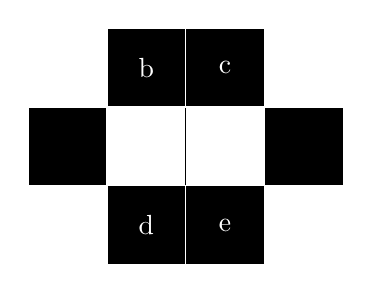
\begin{tikzpicture}
		\path[draw=black,fill=white] (0,0) rectangle (1,1);
		\path[draw=black,fill=white] (1,0) rectangle (2,1);
		\path[draw=white,fill=black] (-1,0) rectangle (0,1);
		\path[draw=white,fill=black] (0,1) rectangle (1,2);
		\path[draw=white,fill=black] (0,-1) rectangle (1,0);
		
		\path[draw=white,fill=black] (2,0) rectangle (3,1);
		\path[draw=white,fill=black] (1,1) rectangle (2,2);
		\path[draw=white,fill=black] (1,-1) rectangle (2,0);
		
		\node[text=white,align=center] at (0.5,1.5) {b};
		\node[text=white,align=center] at (1.5,1.5) {c};
		\node[text=white,align=center] at (0.5,-0.5) {d};
		\node[text=white,align=center] at (1.5,-0.5) {e};
	\end{tikzpicture}
\end{figure}
Now we recognize that the pairs of $b$ and $c$, and $d$ and $e$, are just like the pair $S$ and $a$. Thus, we can continue the pattern up and down arbitrarily. This forms an alternating stripe 2 cells wide. The beauty of such a stripe is that the sides of it can fit into an existing checkerboard pattern. See figure \ref{0PowStripes} for examples.
\begin{theorem}
There cannot be both horizontal and vertical stripes on a $0$-power UPC.
\end{theorem}
\begin{proof}
Suppose you could have both. They would intersect somewhere, which would break the extending-upwards part of the construction because $b$ and $c$ would be on different sides.
\end{proof}
\begin{lemma}
\label{pairsLemma}
The number of adjacent pairs of cells that have different different sides in a given row must be even.
\end{lemma}
\begin{proof}
The number of cells of a given side in a given row is given by the equation:
\begin{equation}
  \label{eqn:pairs}
  n = \frac{2S+D}{2}=S+\frac{D}{2}
\end{equation}
Where $S$ is the number of adjacent pairs with two cells of the same side as is being considered, and $D$ is the number of adjacent pairs with cells of different sides. The division by two comes from double-counting each cell, since they're all part of two pairs. \\
Suppose there were an odd number of adjacent pairs of cells with different sides. Then by equation \ref{eqn:pairs}, there must be a fractional number of cells, which is impossible.
\end{proof}
\begin{theorem}
Consider a 0-power UPC. Without loss of generality, let any stripes be vertical. If there is an even number of stripes, the torus must have an even width. Inversely, if there are an odd number of stripes, it must have an odd width.
\end{theorem}
\begin{proof}
On a given row of a checkerboard configuration $n$ cells wide, you have $n$ pairs of cells on different sides. Each stripe removes one of these pairs. Hence by lemma \ref{pairsLemma}. %FINISH?
\end{proof}

\begin{figure}
  \centering
  \begin{subfigure}[b]{\linewidth}
    \centering
    \fbox{\includegraphics[width=0.5\linewidth]{0config.png}}
    \caption{A $0$-power UPC on a 12-by-12 torus with two stripes}
  \end{subfigure}
  \begin{subfigure}[b]{\linewidth}
    \centering
    \fbox{\includegraphics[width=0.5\linewidth]{0config1stripe.png}}
    \caption{A $0$-power UPC on an 11-by-12 torus with one stripe}  
  \end{subfigure}
  \caption{}
  \label{0PowStripes}
\end{figure}



% DIMENSIONS OF POW 0
\par
Thus, 0-power UPCs can be made on any even-by-even or odd-by-even torus.

\par
% UPC OF 1/3 POWER
We will now consider the most interesting of UPCs. % REASONS WHY THEY'RE INTERESTING
\begin{theorem}
\label{13evenThm}
$\frac{1}{3}$-power UPCs must have an equal number of cells of both sides.
\end{theorem}
\begin{proof}
We will count the numbers of cell neighbors of each side. Every cell in a $\frac{1}{3}$-power UPC has two neighbors of each side; two strong and two weak. Thus, no matter how many cells' neighborhoods are counted, there will be equal numbers of strong and weak neighbors. However, each cell has to have been counted four times by all four of its neighbors. Therefore there must be equal numbers of cells of both sides. 

% DEFINE PAIR?
% FINISH PROOF! (COUNT NEIGHBORS OFF)
% 
\end{proof}
\begin{corollary}
UPCs of power $\frac{1}{3}$ cannot exist on boards with an odd number of cells.
\end{corollary}
\begin{corollary}
All $x$-by-$y$ boards where both $x$ and $y$ are odd do not have any $\frac{1}{3}$-power UPCs. 
\end{corollary}
% HYPOTHESIZE INVERSE (CAN BE PROVEN TO EXIST WITH CONSTRUCTION OF 1-STRIPES)
\begin{theorem}
All $x$-by-$y$ grids where $x$ and $y$ are not both odd has at least one $\frac{1}{3}$-power UPC.  
\end{theorem}
\begin{proof}
All boards with at least one even dimension can have a \textit{1-stripe} configuration (see figure \ref{3PowStripes}). The first step in constructing such a configuration is to choose one of the even dimensions. Fill the columns of that dimension with alternating sides. This will form a sequence of columns, with each column being sandwiched between two columns of the opposite side. This ensures that every cell has two neighbors on the opposite side from the adjacent columns, and two neighbors on the same side above and below it in the column.
% CONSTRUCTION!
\begin{example}
% EXAMPLE OF 1-stripes
\begin{figure}
  \centering
  \fbox{\includegraphics[width=0.5\linewidth]{1-stripes.png}}
  \caption{An example of a 1-stripes configuration on a 16-by-12 torus}
  \label{3PowStripes}
\end{figure}
\begin{remark}
Because of symmetry of side, two opposite configurations can be constructed this way. As well, Boards with two even dimensions will have double the configurations, since they have two choices of dimension to make the columns in. 
\end{remark}
\end{example}
\end{proof}

\par
See table \ref{Empirical3UPCs} for the empirical data on the numbers of different $\frac{1}{3}$ UPCs for different dimensions.
% TABLE WITH NUMBERS OF 1/3 POWER UPCS OF A GIVEN DIMENSION
% SHOULD I REPLACE THE "-"S WITH 0'S?
\begin{table}
\begin{tabular}{l r | *{9}{r} }
  & & y dimension & & & & & & \\
  & & 2 & 3 & 4 & 5 & 6 & 7 & 8 & & 10\\ \hline
  x dimension & 2 & 1 & 1 & 2 & 1 & 2 & 1 & 2 \\
  & 3 & 1 & - & 1 & - & 2 & - & 1 \\
  & 4 & 2 & 1 & 4 & 1 & 2 & 1 & 5 \\
  & 5 & 1 & - & 1 & - & 1 & - & 1 \\
  & 6 & 2 & 2 & 2 & 1 & 5 & 1 & 2 \\
  & 7 & 1 & - & 1 & - & 1 & - & 1 \\
  & 8 & 2 & 1 & 5 & 1 & 2 & 1 & 18 \\
  & \\
& 10 & & & & & & & & & 28 \\
\end{tabular}
\caption{}
\label{Empirical3UPCs}
\end{table}
%CONSIDERATIONS OF POSSIBLE DIMENSIONS
The diagonal of table \ref{Empirical3UPCs} is of particular interest. At the time of writing, these first 5 terms do not appear in any sequence on the OEIS. \\

\par Figure \ref{All3rd} shows all the constant $\frac{1}{3}$-power configurations for 10-by-10. 

\begin{proposition}
There are three other classes of $\frac{1}{3}$-power UPCs. They are as follows: concentric squares, \textit{staircases}, and exotic. \\
\begin{itemize}
  \item Concentric squares are configurations on $4n$-by-$4n$ tori. They are constructed by tessellating a subconfiguration of concentric squares, alternating sides as you tessellate. This subconfiguration is made by starting with a 2-by-2 square, and alternating sides while adding a border, up to a maximum size of $2n$-by-$2n$. See figure \ref{CCircles}.
  \begin{figure}
    \centering
    \fbox{\includegraphics[width=0.25\linewidth]{ccircles.png}}
    \caption{A concentric cicles configuration}
    \label{CCircles}
  \end{figure}
  \item Staircase configurations involve a continuous path of cells following a repeating pattern of \emph{rights} and \emph{ups}. See figure \ref{Staircase}.
  \begin{figure}
    \centering
    \fbox{\includegraphics[width=0.25\linewidth]{3rdData10x10_26.png}}
    \caption{A staircase configuration}
    \label{Staircase}
  \end{figure}
  \item Exotic configurations are all other configurations. Not much is known about them. They typically combine squares and paths. See figure \ref{Exotic}.
  \begin{figure}
    \centering
    \fbox{\includegraphics[width=0.25\linewidth]{3rdData10x10_16.png}}
    \caption{An exotic configuration}
    \label{Exotic}
  \end{figure}
\end{itemize}
% ELABORATE

\end{proposition}


\begin{figure}
  \begin{tabular}{ c | c | c | c }
  \includegraphics[width=0.2\linewidth]{3rdData10x10_1.png} & \includegraphics[width=0.2\linewidth]{3rdData10x10_2.png} & \includegraphics[width=0.2\linewidth]{3rdData10x10_3.png} & \includegraphics[width=0.2\linewidth]{3rdData10x10_4.png} \\ \hline
  \includegraphics[width=0.2\linewidth]{3rdData10x10_5.png} & \includegraphics[width=0.2\linewidth]{3rdData10x10_6.png} & \includegraphics[width=0.2\linewidth]{3rdData10x10_7.png} & \includegraphics[width=0.2\linewidth]{3rdData10x10_8.png} \\ \hline
  \includegraphics[width=0.2\linewidth]{3rdData10x10_9.png} & \includegraphics[width=0.2\linewidth]{3rdData10x10_10.png} & \includegraphics[width=0.2\linewidth]{3rdData10x10_11.png} & \includegraphics[width=0.2\linewidth]{3rdData10x10_12.png} \\ \hline
  \includegraphics[width=0.2\linewidth]{3rdData10x10_13.png} & \includegraphics[width=0.2\linewidth]{3rdData10x10_14.png} & \includegraphics[width=0.2\linewidth]{3rdData10x10_15.png} & \includegraphics[width=0.2\linewidth]{3rdData10x10_16.png} \\ \hline
  \includegraphics[width=0.2\linewidth]{3rdData10x10_17.png} & \includegraphics[width=0.2\linewidth]{3rdData10x10_18.png} & \includegraphics[width=0.2\linewidth]{3rdData10x10_19.png} & \includegraphics[width=0.2\linewidth]{3rdData10x10_20.png} \\ \hline
  \includegraphics[width=0.2\linewidth]{3rdData10x10_21.png} & \includegraphics[width=0.2\linewidth]{3rdData10x10_22.png} & \includegraphics[width=0.2\linewidth]{3rdData10x10_23.png} & \includegraphics[width=0.2\linewidth]{3rdData10x10_24.png} \\ \hline
  \includegraphics[width=0.2\linewidth]{3rdData10x10_25.png} & \includegraphics[width=0.2\linewidth]{3rdData10x10_26.png} & \includegraphics[width=0.2\linewidth]{3rdData10x10_27.png} & \includegraphics[width=0.2\linewidth]{3rdData10x10_28.png} \\
  \end{tabular}
  \caption{All $\frac{1}{3}$-power UPCs on a 10-by-10 torus}
  \label{All3rd}
\end{figure}


\subsection{The First Iteration} \label{FirstIter}

% PROBLEM: TALK ABOUT WHICH THINGS WE CAN PREDICT FOR THE FIRST ITERATION

\par
This segment is largely about what happens to a grid with a random distribution of cells after a single iteration. This is a valuable simplification because knowing that it has a random distribution allows us to easily use probabilistic methods to consider the dynamics of the game. We consider a random board to be one where each cell has a certain constant probability $p$ of being strong, and a corresponding probability $q=1-p$ of being weak. If $p$ is not specified, we take it to be $0.5$.

% ELABORATE ON RANDOMNESS

\begin{definition}[Subconfiguration Proportion (SP)] % DEFINE AS JUST A TUPLE?
This is a tuple containing the numbers of various subconfigurations.%, and is an element of an SPS. Addition is accomplished by piecewise addition of the counts of the subconfigurations.
% SHOULD THIS BE A FUNCTION FROM SUBCONFIGS TO [0,1]
% element of the above space
\end{definition}


% define higher-order variables (e.g. 2-square proportion, change)
\begin{definition}[Subconfiguration Proportion Space (SPS)]
This is a space of possible subconfiguration proportions.
\end{definition}

\begin{example}
An SPS exists for the proportions of 1-by-2 shapes, counting the incidence of $\mathfrak{w}\mathfrak{w}$, $\mathfrak{w}\mathfrak{s}$, $\mathfrak{s}\mathfrak{w}$, and $\mathfrak{s}\mathfrak{s}$. It has three different subconfigurations, and so is trivially a subset of 
$\{ \left(x,y,z\right) \in [0,1]^3 : x+y+z=1 \}$
\end{example}

%
%  MAKE PICTURES OF TOY EXAMPLES AND CONNECT THEM TO THE TUPLES!
%
%

\begin{example}
$\left( \frac{1}{4} , \frac{3}{4} \right) $ could be a subconfiguration proportion for the SPS of single cells.

\end{example}

\begin{definition}[Ratio function]
A ratio operator $R$ is a function from a game $G$ to a subconfiguration proportion. Each SPS has an associated ratio operator.
\end{definition}

\begin{example}
Consider a board with a checkerboard pattern of $\mathfrak{w}$ and $\mathfrak{s}$. The ratio operator for the SPS of individual cells would return $\left(\frac{1}{2},\frac{1}{2}\right)$.
\end{example} % EXPAND EXAMPLE

\begin{definition}[Ratio chain]
A ratio chain is a matrix $C$ representing a Markov chain that acts on a subconfiguration proportion vector.
\end{definition}

\begin{proposition}
For any SPS, associated ratio operator $R$, and game $G$, there exists a ratio chain $C$ with associated error distribution $E$ such that
%CR(G)=R(IG)+\vec{\delta}+\vec{\epsilon}
\begin{equation}
	CR\left(G\right)-R\left(IG\right) \sim E
\end{equation}
%where $\vec{\delta}$ and $\vec{\epsilon}$ depend on the the SPS, the size of the game's board, the proportions of the subconfigurations, and how randomized the board is.
%entropy? is this part of the proportions?
% Here, $\vec{\delta}$ represents the random variation due to different boards having the same subconfiguration proportions, whereas $\vec{\epsilon}$ represents any bias the markov chain might have.
%Finally, $n$ represents the number of subconfigurations which compose the configuration.
% switch epsilon and delta?
% OR SHOULD THESE BE DEFINED AS DISTRIBUTIONS?

\end{proposition}
\begin{proof}
You can always make a trivial matrix to do it. Make the diagonal of the matrix the ratios between before and after proportions. This ratio chain would correspond to an error distribution of constant 0.	
\end{proof}
\begin{example}

\end{example}
This leaves us with questions about two things:
\begin{enumerate}
	\item{\textbf{The Ratio Chain:} How can we construct such a ratio chain? Can we approximate it? Is there an optimal construction?}
	\item{\textbf{The Error:} How can we determine the error distribution $E$? Is it possible to minimize it?}
\end{enumerate}

\par
Both of these questions have several approaches. One can determine a ratio chain for a single iteration by simply constructing a matrix which gives the correct before and after SPs. This ratio chain would be pointless and non-predictive since it could only be constructed by knowing empirically what the next iteration would look like. What we would prefer would be to find as general a way to construct a ratio chain: one which requires as little information as possible to successfully predict the dynamics of the SPS for that game.
%\par
%The first of these questions  % CONTINUE?
%\par
%The second question, how to determine the error, is similar to the first insofar as there are different approaches with varying degrees of empiricism. 


% ALGEBRA OUT HOW TO COMPOUND THIS OVER TIME

% HOW THIS CAN BE USED TO SUCCESSFULLY PREDICT THE FIRST ITERATION
\par
There exists a simple and intuitive way to construct a ratio chain for predicting the first iteration of a random board. It involves enumerating all possible neighborhoods of the SPS subconfigurations, and noting down with what proportions certain subconfigurations change into others. This works because the board is randomized, so each neighborhood has an easily calculable probability. The error in this case is a multidimensional binomial distribution. % is it?

\subsubsection{1-square Proportions}
\par
A 1-square is equivalent to a single cell. There are two possible states that a 1-square can be in, black or white, $\mathfrak{s}$ or $\mathfrak{w}$. The 1-square proportion is a tuple of the percentages of each state of 1-square on the board.
% definition
% cases
% delta
\par
% FIND THE PROBABILITY THAT A RANDOM CELL CHANGES COLOUR
Consider the closed 2-neighborhood of a cell. Without loss of generality we can fix the center cell's side. Now, there are $2^{12}$ possible states of this neighborhood. Let $p$ be the proportion of the selected side.
% COME UP WITH BETTER VARIABLE NAMES
\begin{equation}
P(S)=\frac{\sum^{12}_{i=0}{\left( s_i \right)p^i \left(1-p\right)^{12-i}}}{2^{12}}=1-P(C)
\end{equation}
\begin{equation}
P(C)=\frac{\sum^{12}_{i=0}{\left( c_i \right)p^i \left(1-p\right)^{12-i}}}{2^{12}}=1-P(S)
\end{equation}
Where $S$ and $C$ are the events that the center cell stays the same or changes, $s_i$ is the number of configurations of the 2-neighborhood with $i$ cells of the center's side which \emph{don't} lead to the center cell changing in the next iteration, and $c_i$ is the number of configurations of the 2-neighborhood with $i$ cells of the center's side which \emph{do} lead to the center cell changing in the next iteration.
% CONSIDER THE SAMPLING DISTRIBUTION OF THAT PROPORTION WITH THE-NUMBER-OF-CELLS SAMPLES

% instability
\par
Consider the transition probabilities for a 1-square for the first iteration, generated probabilistically. If we consider the proportion of one side, and what it will be in the next iteration, we see that having equal amounts of both sides appears to be an unstable equilibrium. See figure \ref{fig:cellFirst}.
\begin{figure}
	\centering
	\includegraphics[width=\linewidth]{firstIterationCell.png}
	\caption{}
	\label{fig:cellFirst}
\end{figure}
\par 
This is intriguing, because in general (see \ref{LongTermB} for more) having a 50-50 split of sides seems not only to be a stable equilibrium, but a sink to which only the most extreme proportions are not attracted to.
\par
As for the error in predicted proportion, we can calculate this using a binomial distribution. If there are $n$ cells and we know that the probability that a square will stay the same in the next iteration is $P(S)$, then the variance in the number of cells staying the same is $nP(S)(1-P(S))$. Thus, the standard deviation of that number is $\sqrt{nP(S)(1-P(S))}$, and thus the standard deviation of the proportion of cells staying the same is $\sqrt{\frac{P(S)(1-P(S))}{n}}$. One can do similarly for the changing cells, and from this calculate the standard deviation in proportions of both sides.
\subsubsection{2-square Proportions} \label{2squareFirst}
\par
2-Square subconfigurations are possible states of 2-by-2 squares. There are 16 such subconfigurations, but usually we consider the subconfigurations up to rotational symmetries leaving us with 6 possible states, seen in figure \ref{2Shapes}.

\begin{figure}
  \centering
  \begin{subfigure}[b]{0.3\linewidth}
    \fbox{\includegraphics[width=\linewidth]{side.png}}
    \caption{Side}
  \end{subfigure}
  \begin{subfigure}[b]{0.3\linewidth}
    \fbox{\includegraphics[width=\linewidth]{diag.png}}
    \caption{Diagonal}
  \end{subfigure}
  \begin{subfigure}[b]{0.3\linewidth}
    \fbox{\includegraphics[width=\linewidth]{blackCorner.png}} % I switched back to the old definition of black corner after making this file
    \caption{White Corner}
  \end{subfigure}
  \begin{subfigure}[b]{0.3\linewidth}
    \fbox{\includegraphics[width=\linewidth]{whiteCorner.png}}
    \caption{Black Corner}
  \end{subfigure}
  \begin{subfigure}[b]{0.3\linewidth}
    \fbox{\includegraphics[width=\linewidth]{whiteSquare.png}}
    \caption{White Square}
  \end{subfigure}
  \begin{subfigure}[b]{0.3\linewidth}
    \fbox{\includegraphics[width=\linewidth]{blackSquare.png}}
    \caption{Black Square}
  \end{subfigure}
  \caption{2-square states}
  \label{2Shapes}
\end{figure}

\par
Here are some pictures with various types of subconfigurations coloured.
\begin{figure}
  \centering
  \begin{subfigure}[b]{0.3\linewidth}
    \fbox{\includegraphics[width=\linewidth]{img0019Coloured2.png}}
    \caption{Sides}
  \end{subfigure}
  \begin{subfigure}[b]{0.3\linewidth}
    \fbox{\includegraphics[width=\linewidth]{img0019Coloured3.png}}
    \caption{Diagonals}
  \end{subfigure}
  \begin{subfigure}[b]{0.3\linewidth}
    \fbox{\includegraphics[width=\linewidth]{img0019Coloured4.png}}
    \caption{White Corner}
  \end{subfigure}
  \begin{subfigure}[b]{0.3\linewidth}
    \fbox{\includegraphics[width=\linewidth]{img0019Coloured5.png}}
    \caption{Black Corner}
  \end{subfigure}
  \begin{subfigure}[b]{0.3\linewidth}
    \fbox{\includegraphics[width=\linewidth]{img0019Coloured0.png}}
    \caption{White Squares}
  \end{subfigure}
  \begin{subfigure}[b]{0.3\linewidth}
    \fbox{\includegraphics[width=\linewidth]{img0019Coloured1.png}}
    \caption{Black Squares}
  \end{subfigure}
  \caption{2-square samples from a 12-by-12 torus simulation}
\end{figure}

\par
If we have a random board, then we can easily consider what the starting proportions of these subconfigurations should be. 
\begin{table}[H]
\label{InitPropsTable}
\begin{tabular}{r | l}
  Shape & Expected Starting Proportion \\ \hline
  Side & $\frac{1}{4}$ \\
  Diagonal & $\frac{1}{8}$ \\
  White Corner & $\frac{1}{4}$ \\
  Black Corner & $\frac{1}{4}$ \\
  White Square & $\frac{1}{16}$ \\
  Black Square & $\frac{1}{16}$ \\
\end{tabular}
\caption{}
\end{table}

\par
The problem now is to predict what the proportions of these 6 subconfigurations will be in the next iterations. To accomplish this, we will construct a ratio chain. To construct this chain:
\begin{enumerate}
  \item{} Consider the 2-neighborhood around a 2-square (see figure \ref{2Neighborhood})
  \begin{figure}
    \label{2Neighborhood}
    \caption{2-neighborhood around a 2-square marked by '$c$'s}
    \centering
    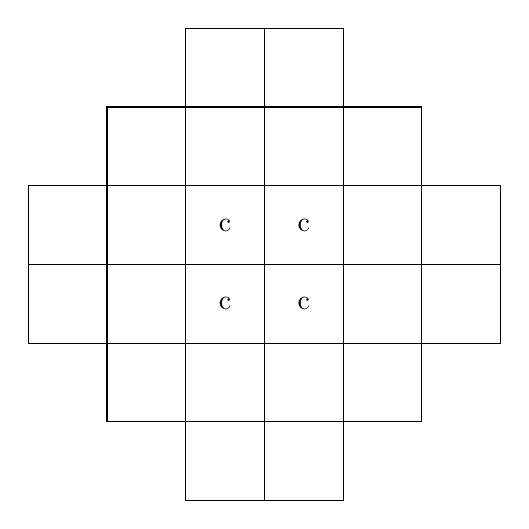
\begin{tikzpicture}
      \foreach \i in {2,...,3} {
        \draw(\i,0) rectangle (1+\i,1);
      }
      \foreach \i in {1,...,4} {
        \draw(\i,1) rectangle (1+\i,2);
      }
      \foreach \i in {0,...,5} {
        \draw(\i,2) rectangle (1+\i,3);
      }
      \foreach \i in {0,...,5} {
        \draw(\i,3) rectangle (1+\i,4);
      }
      \foreach \i in {1,...,4} {
        \draw(\i,4) rectangle (1+\i,5);
      }
      \foreach \i in {2,...,3} {
        \draw(\i,5) rectangle (1+\i,6);
      }
      \node at (2.5,2.5) {c};
      \node at (3.5,2.5) {c};
      \node at (3.5,3.5) {c};
      \node at (2.5,3.5) {c};
      %\path[draw=white,fill=black] (2,\i) rectangle (3,1+\i);
    \end{tikzpicture}    
  \end{figure}
  \item{} For all 6 different subconfigurations:
  \begin{enumerate}
    \item{} For all $2^{20}$ possible neighborhoods:
    \begin{enumerate}
      \item{} Place the subconfiguration in the center of the neighborhood.
      \item{} Iterate once.
      \item{} Record which subconfiguration is now in the center.
    \end{enumerate}
    \item{} Divide the counts of the final subconfigurations by $2^{20}$ to normalize them.
  \end{enumerate}
  
\end{enumerate}
The Markov chain generated by this is the following:
\begin{equation}
  \begin{bmatrix}
  (\texttt{white squares})' \\
  (\texttt{black squares})' \\
  (\texttt{side})' \\
  (\texttt{diag})' \\
  (\texttt{white corner})' \\
  (\texttt{black corner})'
  \end{bmatrix}
  =
  \begin{bmatrix}
  0.815 & 0.000 & 0.069 & 0.105 & 0.005 & 0.422 \\
  0.000 & 0.820 & 0.069 & 0.105 & 0.422 & 0.005 \\
  0.020 & 0.020 & 0.643 & 0.196 & 0.127 & 0.127 \\
  0.006 & 0.006 & 0.001 & 0.115 & 0.006 & 0.006 \\
  0.003 & 0.155 & 0.108 & 0.239 & 0.408 & 0.033 \\
  0.155 & 0.003 & 0.108 & 0.239 & 0.033 & 0.408 
  \end{bmatrix}
  \begin{bmatrix}
  (\texttt{white squares}) \\
  (\texttt{black squares}) \\
  (\texttt{side}) \\
  (\texttt{diag}) \\
  (\texttt{white corner}) \\
  (\texttt{black corner})
  \end{bmatrix}
\end{equation}

Which when applied to the initial conditions in table \ref{InitPropsTable} gives us the proportions for iteration 2 of a random board:
\begin{table}[H]
\label{SecondPropsTable}
\begin{tabular}{r | l}
  Shape & Predicted Iteration 2 Proportion \\ \hline
  Side & 0.251 \\
  Diagonal & 0.018 \\
  White Corner & 0.177 \\
  Black Corner & 0.177 \\
  White Square & 0.188 \\
  Black Square & 0.188 \\
\end{tabular}
\caption{}
\end{table}

Which is supported by the empirical evidence. % ELABORATE!

%huge section
\subsection{Long Term Behavior}
\label{LongTermB}
% HAVE BLURB ABOUT WHY LONG-TERM
\par
There are many reasons why we should consider the long-term behavior of the game. The first being that it represents an averaged or compounded version of the game rules. Another is learning about local versus global structure.

\begin{definition}[Long-Term Configuration (LTC)]
Any configuration which 
\end{definition}

% REMEMBER TO GO THROUGH AND CHANGE EVERYTHING TO LTC

\par
The LTCs seem fairly random, but the board is noticeably different, as shown in figure 18.% \ref{BeforeAfter}.
% TODO fix this static figure number!

% PICTURES OF BEFORE AND AFTER
\begin{figure}
  \label{BeforeAfter}
  \centering
  \begin{subfigure}[b]{0.45\linewidth}
    \fbox{\includegraphics[width=\linewidth]{before.png}}
    \caption{random starting configuration}
  \end{subfigure}
  \begin{subfigure}[b]{0.45\linewidth}
    \fbox{\includegraphics[width=\linewidth]{after.png}}
    \caption{long-term configuration}
  \end{subfigure}
  \caption{}
\end{figure}

\subsubsection{Threshold for Homogeneous Stability} \label{HomoStability}
% DEFINE HOMOGENEOUS STABILITY?
\par
Recall from \ref{SpecialShapes} that the L, I, and O tetrominoes are parastable. These are the smallest parastable patterns. By the nature of their parastability, they can "re-seed" a grid with very few of a given side. Thus, we can make a probabilistic argument for the cutoff below which the proportion between strong and weak should not be able to return to 50/50.

\par
These three types of tetrominoes have 11 different configurations, because of their symmetries.
% PUT IN OTHER PARAGRAPH?
\par
Let $X$ be the number of parastable tetrominoes on a torus with
width $n$ and height $m$, and $\{X_{i,j}:i\in\{1,\ldots,n\},j\in\{1,\ldots,m\}\}$
be the indicator variables for there being a parastable tetromino at
position $\left(i,j\right)$. Finally, let $p$ be the proportion of cells
on the torus with the given side. Then
\begin{equation}
	E(X_{i,j})=11p^4
	\end{equation}
And so by linearity of expected value
\begin{equation}
	E(X)=\sum_{i=1}^n \sum_{j=1}^m E(X_{i,j})=\sum_{i=1}^n \sum_{j=1}^m 11p^4 = 11nmp^4
\end{equation}
Thus, the critical proportion such that we expect there to be one
parastable tetromino is $p=\left(\frac{1}{11nm}\right)^{\frac{1}{4}}$.
\par
We can see the empirical evidence for this in figure \ref{HomoDiagrams}.

\begin{figure}
  \centering
  \begin{subfigure}[b]{0.6\linewidth}
    \fbox{\includegraphics[width=\linewidth]{homostableData25x25x25.png}}
    \caption{25-by-25 torus. Expected crossover at ${p=\frac{1}{11\times25\times25}}^{\frac{1}{4}}=0.110$}
  \end{subfigure}
  \begin{subfigure}[b]{0.6\linewidth}
    \fbox{\includegraphics[width=\linewidth]{homostableData50x50x25.png}}
    \caption{50-by-50 torus. Expected crossover at ${p=\frac{1}{11\times50\times50}}^{\frac{1}{4}}=0.077$}
  \end{subfigure}
  \begin{subfigure}[b]{0.6\linewidth}
    \fbox{\includegraphics[width=\linewidth]{homostableData100x100x25.png}}
    \caption{100-by-100 torus. Expected crossover at ${p=\frac{1}{11\times100\times10}}^{\frac{1}{4}}=0.055$}
  \end{subfigure}
  \caption{}
  \label{HomoDiagrams}
\end{figure}

\subsubsection{Behaviour of Power} \label{Power}

\par
The average power of a grid usually increases over time to approach an asymptote. This makes sense intuitively; A more powerful subconfiguration will change its neighbors and not change itself similar to natural selection, or so the intuition goes.

\par
To delve more into the asymptote, we look to figure \ref{AveragePower}. We see that just as the intuition would have, average power increases roughly monotonically. The asymptotic average power seems to be about $0.275$. Why it is this value in particular remains an open problem.

\begin{figure}
  \caption{}
  \label{AveragePower}
  \centering
  \includegraphics[width=0.75\linewidth]{AveragePower.png}
\end{figure}

\par
Perhaps to understand power better we must not look simply at the average power. Figure \ref{PowerDist} shows the numbers of cells with different powers. In the long-term, $\frac{1}{3}$ dominates, followed by $\frac{1}{4}$, with $\frac{1}{5}$ and $0$ taking third and fourth; A simple ordering of highest power means highest proportion. An interesting question, however, is how those powers get to their final proportions. At the start, $\frac{1}{4}$ and $\frac{1}{5}$ jump up significantly before slowly decaying to their equilibria. $\frac{1}{4}$ even surpasses $\frac{1}{3}$ for a dozen iterations. $\frac{1}{3}$ and $0$, on the other hand, both jump down at the beginning. $\frac{1}{3}$ then begins its slow growth to the top, but $0$ continues downward.

\par
These peculiarities showcase how local behavior does not necessarily favor stronger subconfigurations. Rather, only on the aggregate do stronger subconfigurations win out in the end. This will be discussed more in section \ref{GlobalLocal}.

\begin{figure}
  \caption{}
  \label{PowerDist}
  \centering
  \includegraphics[width=0.75\linewidth]{PowerDist.png}
\end{figure}

\subsubsection{2-square Proportions} \label{LongTerm2P}
%Show why 3-3 not as important via entropy
%TALK ABOUT WHY IT IS INTERESTING THAT THE PROPORTIONS ARE THE SAME FOR RANDOM SEEDS AND PARASTABLE STARTS

\par
Recall from section \ref{2squareFirst} the definition of a 2-square. Similar to \ref{2squareFirst}, this section will deal with the \emph{subconfiguration proportions} of 2-squares. To start off let us simply look at an example of the subconfiguration proportions of a random grid over time in figure \ref{2SquaresOverTime}.

\begin{figure}
  \centering
  % MAKE THE TITLES ON THIS GRAPH LARGER!
  % ALSO EXPLAIN WHAT'S GOING ON FOR ONLY-READERS AND IF NOT COLOUR
  \includegraphics[width=0.75\linewidth]{LTC2Squares.png}
  \caption{2-square proportions on a 300-by-300 torus over time}
  \label{2SquaresOverTime}
\end{figure}

\par
The first thing we notice looking at figure \ref{2SquaresOverTime} is that sides slowly but steadily increase to one third of the board, and are the most common subconfiguration. Diagonals are the next simplest subconfiguration, jumping down significantly in the first iteration then slowly increasing to an asymptote of one fiftieth of the board. Finally we have squares and corners. Both of these subconfigurations come in two variants, but it is uncommon that their proportions vary much. 

\par
The subconfigurations with side variants, squares and corners, have several interesting properties. First, they perform a strange oscillation during the first several iterations. Initially we thought this \emph{blip} was merely an accident, but it is consistently present. Secondly, we have hypothesized that any initial asymmetries in squares persist. This can be seen more readily in the parastable case (see figure \ref{ParaLongTerm}). However not much research has been done on this. 

\par
Extracting from figure \ref{2SquaresOverTime} we find the empirical long-term 2-square proportions.

\begin{table}[H]
\begin{tabular}{r|l}
  Shape & Final Proportion \\ \hline
  Side & 0.334 \\
  Diagonal & 0.020 \\
  White Corner & 0.188 \\
  Black Corner & 0.188 \\
  White Square & 0.135 \\
  Black Square & 0.135 \\  
\end{tabular}
\caption{}
\end{table}

\par
One interesting thing is how these same long-term proportions seem to be shared by parastable configurations (see figure \ref{ParaLongTerm}).

% ELABORATE!!!

\begin{figure}
  \label{ParaLongTerm}
  \centering
  \includegraphics[width=0.75\linewidth]{ParaLTC2Squares.png}
  \caption{2-square proportions on a 300-by-300 starting with only a black 2-square surrounded by white cells}
\end{figure}

\par
The variables of 1-2 and 2-2 proportion are intriguing because they directly disprove the hypothesis that the distribution of large subconfigurations is predictable by their smaller subsubconfigurations' proportions. % REWRITE THIS LINE?


% TALK ABOUT HOW MUCH IT DID WORK AND HOW MUCH IT DIDN'T
\par
Recall the ratio chain used to model the proportion of 2-squares in section \ref{2squareFirst}. If we apply this ratio chain continuously, we arrive at the following stable state:
\begin{table}
\begin{tabular}{r|l}
  Shape & Ratio Chain Stable State Proportion \\ \hline
  Side & 0.122 \\
  Diagonal & 0.006 \\
  White Corner & 0.116 \\
  Black Corner & 0.116 \\
  White Square & 0.320 \\
  Black Square & 0.320 \\
\end{tabular}
\caption{}
\end{table}
% SHOULD I PLACE THE OTHER DATA BESIDE THIS?

\par
If we compare these data to the empirical long-term proportions, we get some mixed results.

\begin{table}[H]
\begin{tabular}{r|c c c | l}
  Shape & Actual Starting & Actual Final & Ratio Chain Final & Final Error \\ \hline
  Side & 0.250 & 0.334 & 0.122 & -0.212 \\
  Diagonal & 0.125 & 0.020 & 0.006 & -0.014 \\
  White Corner & 0.250 & 0.188 & 0.116 & -0.072 \\
  Black Corner & 0.250 & 0.188 & 0.116 & -0.072 \\
  White Square & 0.062 & 0.135 & 0.320 & 0.185 \\
  Black Square & 0.062 & 0.135 & 0.320 & 0.185 \\
\end{tabular}
\caption{}
\end{table}
\par The first thing that you will notice is that the ratio chain gets the long-term proportions significantly wrong. However, there is also an interesting trend. With the exception of sides, every proportion moves "in the right direction". Diagonals decrease significantly, and the ratio chain reflects this. The corners decrease slightly, and the ratio chain reflects this. The squares increase significantly, and the ratio chain reflects this. In all these cases, the ratio chain appears to simply \emph{overshoot} its target.

\par
After this, we tried several tweaks to the method of generating the ratio chain. Initially we thought it was a problem of needing to weigh the different possible neighborhoods. We tried weighing the probability contribution of each neighborhood by $e^{|(\vec{e}-\vec{a}|}$, where $e$ was the expected 2-2 proportion SP of the neighborhood and $a$ was the actual SP of the neighborhood being considered. This did not work as well as expected either.
% MAYBE PUT IN THE ACTUAL CHAIN

\par
Finally, we decided that the most foolproof method of constructing a ratio chain for long-term 2-2 proportions would be to simply sample the transition probabilities of randomly sampled 2-squares on boards which had reached their long-term state. For this chain we also considered all 16 possible 2-square subconfigurations, rather than collapsing rotationally equivalent ones. The results of this test were, however, even worse than the original ratio chain. The stable-state solution of the Markov chain was the following:

\begin{table}[H]
\begin{tabular}{r|c c c | l}
  Shape & Actual Starting & Actual Final & Ratio Chain Final & Final Error \\ \hline
  Side         & 0.250 & 0.334 & 0.018 & -0.316 \\
  Diagonal     & 0.125 & 0.020 & 0.115 & 0.095 \\
  White Corner & 0.250 & 0.188 & 0.033 & -0.155 \\
  Black Corner & 0.250 & 0.188 & 0.034 & -0.154 \\
  White Square & 0.062 & 0.135 & 0.394 & 0.259 \\
  Black Square & 0.062 & 0.135 & 0.406 & 0.271 \\
\end{tabular}
\caption{}
\end{table}

% SIGNIFICANCE OF THIS FOR RATIO CHAIN MODELLING

\subsubsection{Stability Over Time}
The game tends to start off chaotic and then grow more stable over time. A simple way to see this is the number of cells that changed in the last iteration decreases over time, towards an asymptote (see figure \ref{ChangeOverTime}). 

\begin{figure}
  \centering
  \includegraphics[width=0.75\linewidth]{changeProps.png}
  \caption{}
  \label{ChangeOverTime}
\end{figure}

% ALSO MENTION HOW POWER IS INVOLVED
\par
Power likely plays an integral role in increasing stability. As was mentioned in section \ref{Power}, the average power of the game increases over time. There are less neighborhoods for a high power cell to change than for a low power one. 

\subsubsection{Cycle length}

% INTRO & EXPLAIN GRAPH & SLOPE
\begin{definition}[pre-cycle length]
This is the number of iterations until the game reaches the first state which is part of the final cycle.
% MAKE THIS BETTER?
\end{definition}
\par
The data from simulations for the pre-cycle length are in figure \ref{Precycle}. 

\begin{figure}
  \centering
  \label{Precycle}
  \includegraphics[width=\linewidth]{precycles.png}
  \caption{Precycle length for random $n$-by-$n$ boards where $5\leq n \leq 100$. Error bars show 1 stdev}
\end{figure} % MENTION HOW THE LINE OVERESTIMATES AT THE SMALL VALUES?

\par
There's an argument here for why the global structure of the game cannot be determined by just the local structure of the game. This is because if the only the local structure mattered, then there should be some finite area around each cell which determines its long-term state, and some corresponding time for that long-term state to be reached. Anything outside that area should not affect it. This would mean that once the board was larger than this area, any larger boards should not affect the time to reach long-term state. Thus, the pre-cycle length should eventually plateau. Perhaps this area is very large, but it seems more likely such an area does not exist.

\par
There is also potentially pertinent information in the slope of the data in figure \ref{Precycle}. Notice that it is about $2.25$. The maximum distance between two points on an $n$-by-$n$ torus is $2n$. Changes in the power-index game generally travel one cell at a time (there are certain special circumstances in which changes can induce changes 2 cells away by increasing the power of their neighbor). So, the fact that it takes just slightly longer than $2n$ iterations for the game to reach its precycle suggests that the starting state of every cell acts like a \emph{ripple}, and once that ripple has passed over every other cell, they can finally take their final states, as no new information is arriving. I hypothesize that it is just a constant number of iterations after all the ripples have finished that every cell takes its final state, and so asymptotically the slope of the pre-cycle against diameter of the torus should be 2.


\subsubsection{The Search for Entropy}
\par
One of the more exotic directions which we explored to try to gain some insight into the long-term behavior of the game was examining the Shannon entropy of various SPSs over time, and their long-term values. We expected the game to move away from random as time went on, and this was borne out by the data. Another surprising result is that the long-term entropy of larger-scale SPSs was lower. % IS THIS SURPRISING?

\subsubsection{Global vs Local} \label{GlobalLocal}
\par
The successes and failures of these attempts at using ratio chains to model the game lead us to a question: To what extent is the behavior of the game determined by local or global structure. Let us elaborate on these two situations.

\par
First, local behavior is behavior determined solely by the cells within some finite area. An example of this is the behavior of a cell over a single iterations, since it is only affected by cells within its 2-neighborhood. Local behavior is nice because it limits the scope which we must examine to determine what will happen.

\par
Global behavior is the opposite of local behavior. It is behavior which depends on the state of the entire game. Changes on one side of the board can affect the other side, no matter how far.

\par
Some phenomena of the power-index game are local while others are global. Parastability on an empty grid (see \ref{EmptyGrid}) is an example of a global phenomena since it reaches out arbitrarily far enough given enough iterations. This is intriguing because there are parastable subconfigurations as small as 4 cells, so having just one on an otherwise empty board can make all the difference in terms of long-term structure. % continue

\par
However, some configurations seem to naturally \emph{insulate} against changes. Changing a single cell on a LTC rarely induces changes that travel very far. The same is also true of $\frac{1}{3}$-power UPCs. Other UPCs don't share this same stability, so this likely stems from them having a lower-than optimal average power.

\par
The pre-cycle length also might contain some clues about the global nature of LTCs. Empirically the pre-cycle length seems to increase linearly with the size of the board. If the long-term state of a cell were determined by some finite area around it, then it should have some set time to stabilize which shouldn't be exceeded just because the board is larger than that area.

% cycle length
% Entropy
% cooling

%\subsection{Some other results}

%Spectrum stuff
%Crystalization (parastability breaking down at 50%-prob-of-changing)
%change space
%transition matrix images

\section{Conclusion}
\par
The Power-Index game has many different interesting phenomena. It is more complex than it appears at first glance. The glider we found reaffirms the earlier result that there was not an upper limit on cycle size, despite the general tendency for the game to "calm down". We also examined many uniform power configurations, which showed just how rich the structures of the game can be. Finally, we tried to crack the code of long-term configurations. This, we did not accomplish, but that only underlines its complexity.

\par
We introduced many new concepts in this paper. Many of them were made in the hope of shedding more light on the larger and longer scale structures of the game. We explored the concept of ratio chains to see how they might be used to model the power-index game in an aggregate way. We found them to be readily applicable in the first implementation. However we discovered many difficulties in extending that applicability to the long-term. Hopefully our attempts will lay the groundwork for future success at that task.

\par
One of the main takeaways of this research is that there are many unexplored frontiers to the power-index game. We have but dipped our toes in the ocean that is enumerating all stable configurations. We have only just started learning how to use ratio chains to simplify modelling the game. We have just scratched the surface of characterizing long-term configurations. But as the proverb goes, \emph{the journey of a thousand miles begins with a single step}.

% 
% RATIO CHAINS
% SHORT TERM
% LONG TERM
% STABILITY


\subsection{Open Problems}
\begin{itemize}
\item
Enumerating all stable subconfigurations on an empty grid (see \ref{EmptyGrid}).
\item
Enumerating all $\frac{1}{3}$ - power stable configurations. This is equivalent to the general problem of colouring cells on a torus such that each cell has two neighbors of each colour. (see \ref{UPCs})
\item
Variance of the threshold for homogeneous stability. (see \ref{HomoStability})
\item
Proof for maximum average power. (see \ref{Power})
\item
Under what circumstances do asymmetries form and persist in square and corner 2-square subconfigurations. (see \ref{LongTerm2P})
\item
Method of constructing a ratio-chain for long-term behavior. (see \ref{LongTerm2P})

\end{itemize}

\subsection{Acknowledgments}
\begin{itemize}
\item \textbf{Jeannette Janssen} and \textbf{Jordan Barrett} for their supervision and guidance. 
\item \textbf{NSERC} for making this all possible through their funding.
\item \textbf{Dalhousie}
\end{itemize}

\bibliographystyle{plain}
\bibliography{./references}{}

\end{document}
